
\begin{frame}{What the heck is quantum gravity anyway?}
 \begin{columns}[onlytextwidth,t]
  \uncover<1->{\begin{column}{0.48\textwidth}
    \begin{block}{Classical Gravity}
     \vspace{0pt}
     Einstein Field equations:
     \begin{align*}
      \uncoverubrace<2->{\frac{8 \pi G}{c^4}}{\kappa}\uncoverubrace<2->{T_{\mu\nu}}{\substack{\text{stuff within} \\  \text{space-time}}} & = \uncoverubrace<2->{R_{\mu\nu} - \frac{1}{2} R g_{\mu\nu} + \Lambda g_{\mu \nu}}{\text{geometry of space-time}}
      \uncover<3->{\intertext{Einstein Hilbert Action (for $T_{\mu\nu} = 0$):}
      S_{EH} [g] & = \frac{1}{2 \kappa} \int \mathrm{d}^4 x \sqrt{-\mathrm{det} \, g} \, (R - 2\Lambda)}
     \end{align*}
    \end{block}
   \end{column}}
  \begin{column}{0.48\textwidth}
   \uncover<4->{\begin{block}{Quantum Gravity}
     \vspace{0pt}
     Path integral formulation:
     \begin{align*}
      Z_E & = \int \mathcal{D} g \, \exp \left( - S[g]\right)
     \end{align*}
    \end{block}}
   \uncover<5->{\textbf{Problems}
    \begin{itemize}
     \item non renormalizable coupling expansion
     \item might still be asymptotically safe \\ $\Rightarrow$ non-pertubative approaches
    \end{itemize}}
  \end{column}
 \end{columns}
\end{frame}


\begin{frame}{Triangulations}
 \begin{columns}
  \begin{column}{0.38\textwidth}
   \begin{block}{Discretisation of $Z_E$}
    \vspace{0pt}
    \uncover<1->{Approximate space-time Manifold by triangulation}
    \uncover<2->{\begin{align*}
      \underbrace{\int \mathcal{D}g}_{\substack{\text{Integral over possible} \\ \text{metric tensors}}} \longrightarrow \underbrace{\sum_T \frac{1}{C_T}}_{\substack{\text{Sum over possible}\\ \text{triangulations}}}
     \end{align*}}
    \uncover<3->{Only equilateral triangles (simplices)}
    \uncover<4->{\begin{align*}
      S_E & = -\kappa_2(\kappa) N_2 + \kappa_4(\kappa, \Lambda) N_4
     \end{align*}
     where $N_k$ is the number of $k$-simplices in  $T$}
   \end{block}
  \end{column}
  \begin{column}{0.60\textwidth}
   \begin{figure}
    \centering
    \only<1-2>{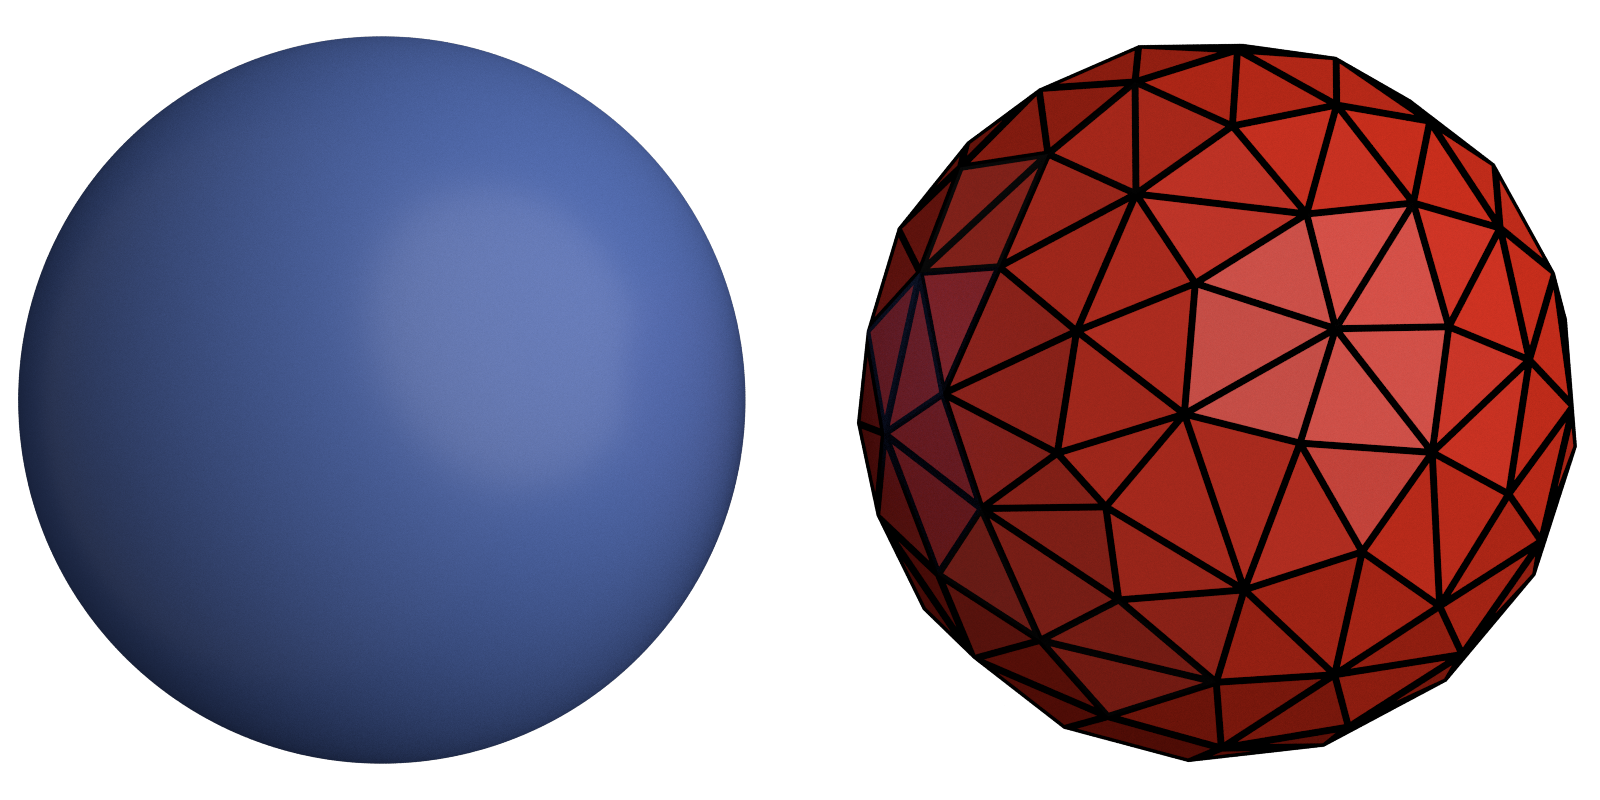
\includegraphics[width=\textwidth]{pics/triangulation-fib.png}
     \caption{Triangulation of $S_2$ obtained by the Fibonacci Lattice\\ \tiny{rendered with the fresnel library (\url{https://github.com/glotzerlab/fresnel})}}}
    \only<3-4>{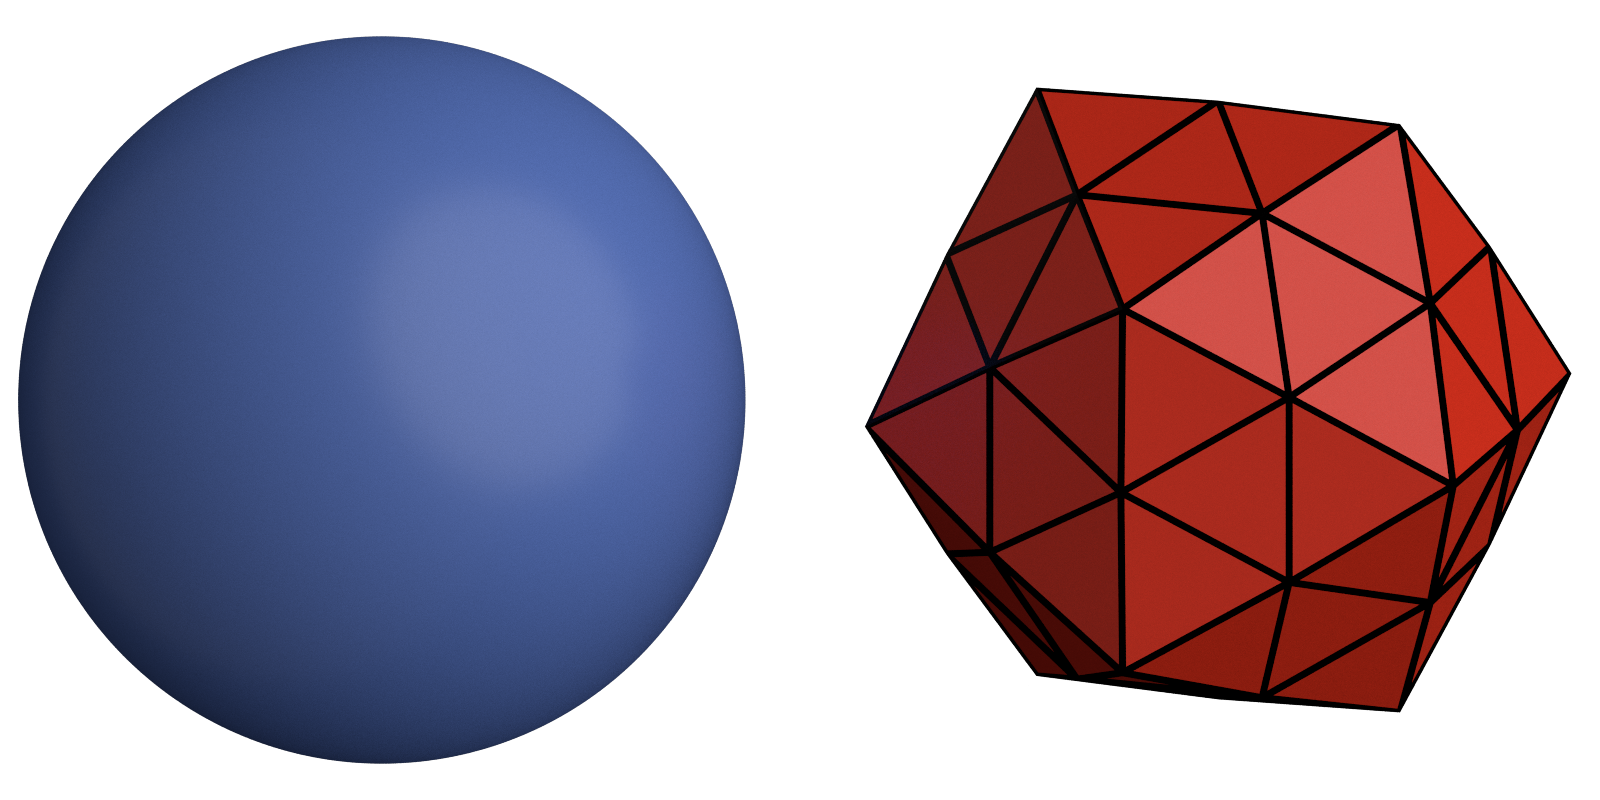
\includegraphics[width=\textwidth]{pics/triangulation-ico.png}
     \caption{Triangulation of $S_2$ obtained from Icosahedron\\ \tiny{rendered with the fresnel library (\url{https://github.com/glotzerlab/fresnel})}}}
   \end{figure}
  \end{column}
 \end{columns}
\end{frame}


\begin{frame}{Pachner Moves}
 %Local Update Moves for Metropolis-Monte-Carlo simulations:
 \begin{columns}[onlytextwidth,t]
  \begin{column}{0.37\textwidth}
   \uncover<1->{\begin{block}{Local Update Moves}
     \vspace{0pt}
     (Some Bullet Points to Explain the ergodic nature of the Pachner moves)
    \end{block}}
  \end{column}
  \begin{column}{0.34\textwidth}
   \begin{block}{2D}
    \vspace{0pt}
    \uncover<2->{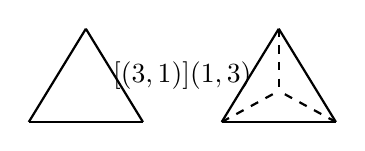
\begin{tikzpicture}
 \def\a{1.45}
 \def\b{0.5}
 \def\trigConst{0.816497}

 %1st Triangle
 \draw[thick] (-\a-\b,0) -- (-\b, 0);
 \draw[thick] (-\a-\b,0) -- ({-\b-(0.5*\a)}, {\trigConst * \a});
 \draw[thick] (-\b,0)    -- ({-\b-(0.5*\a)}, {\trigConst * \a});

 %2nd Triangle
 \draw[thick] (\a + \b,0) -- (\b, 0);
 \draw[thick] (\a+\b,0)   -- ({\b+(0.5*\a)}, {\trigConst * \a});
 \draw[thick] (\b,0)      -- ({\b+(0.5*\a)}, {\trigConst * \a});

 %Lines to center
 \draw[thick, dashed] (\b,0)                             -- ({\b+(0.5*\a)}, {\trigConst * \a * 0.33333});
 \draw[thick, dashed] (\a+\b,0)                          -- ({\b+(0.5*\a)}, {\trigConst * \a * 0.33333});
 \draw[thick, dashed] ({\b+(0.5*\a)},{\trigConst * \a}) -- ({\b+(0.5*\a)}, {\trigConst * \a * 0.33333});

 \node[align=center] at (0,{0.5*\trigConst*\a}) {$\xrightleftharpoons[(3,1)]{(1,3)}$};
\end{tikzpicture}
}\\
    \vspace{1.0em}
    \uncover<3->{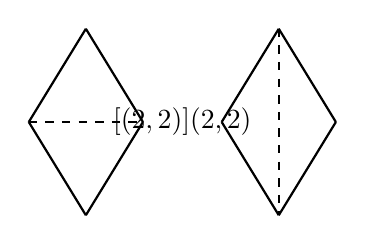
\begin{tikzpicture}
 \def\a{1.45}
 \def\b{0.5}
 \def\trigConst{0.816497}

 %1st Triangle
 \draw[thick, dashed] (-\a-\b,0) -- (-\b, 0);
 \draw[thick] (-\a-\b,0)         -- ({-\b-(0.5*\a)}, {\trigConst * \a});
 \draw[thick] (-\b,0)    -- ({-\b-(0.5*\a)}, {\trigConst * \a});
 \draw[thick] (-\a-\b,0)         -- ({-\b-(0.5*\a)}, {-\trigConst * \a});
 \draw[thick] (-\b,0)            -- ({-\b-(0.5*\a)}, {-\trigConst * \a});


 %2nd Triangle
 \draw[thick, dashed] ({\b+(0.5*\a)}, {\trigConst * \a}) -- ({\b+(0.5*\a)}, {-\trigConst * \a});
 \draw[thick] (\a+\b,0)                                  -- ({\b+(0.5*\a)}, {\trigConst * \a});
 \draw[thick] (\b,0)                                     -- ({\b+(0.5*\a)}, {\trigConst * \a});
 \draw[thick] (\a+\b,0)                                  -- ({\b+(0.5*\a)}, -{\trigConst * \a});
 \draw[thick] (\b,0)                                     -- ({\b+(0.5*\a)}, -{\trigConst * \a});

 %Lines to center

 \node[align=center] at (0,0) {$\xrightleftharpoons[(2,2)]{(2,2)}$};
\end{tikzpicture}
}
   \end{block}
  \end{column}
  \begin{column}{0.27\textwidth}
   \uncover<4->{\begin{block}{3D}
     \vspace{0pt}
     
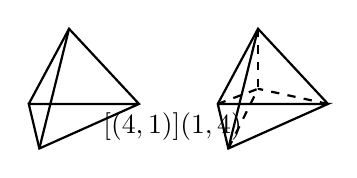
\begin{tikzpicture}[scale=1]
 \def\a{1.40}
 \def\b{0.5}
 \def\trigConst{0.816497}


 \begin{scope} [x     = {(1cm,0)},
   y     = {({0.7cm*cos(135)},{-0.7cm*sin(135)})},
   z     = {(0,1cm)}]

  \path coordinate (T1) at ({-(\b + (0.5*\a))}, {0.3333*\trigConst*\a}, {\trigConst*\a})
  coordinate (A1) at ({-\b},0,0)
  coordinate (B1) at ({-(\a + \b)},0,0)
  coordinate (C1) at ({-(\b + (0.5*\a))},{\trigConst*\a},0);


  \path coordinate (T2) at ({(\b + (0.5*\a))}, {0.3333*\trigConst*\a}, {\trigConst*\a})
  coordinate (A2) at ({\b},0,0)
  coordinate (B2) at ({(\a + \b)},0,0)
  coordinate (C2) at ({(\b + (0.5*\a))},{\trigConst*\a},0)
  coordinate (D2) at ({(\b + (0.5*\a))}, {0.3333*\trigConst*\a}, {0.3333*\trigConst*\a});


  \draw[thick]  (A1)  -- (B1) -- (C1) -- (A1) -- (T1) -- (B1);
  \draw[thick]  (C1) -- (T1);

  \draw[thick]  (A2)  -- (B2) -- (C2) -- (A2) -- (T2) -- (B2);
  \draw[thick]  (C2) -- (T2);

  \draw[thick, dashed] (A2) -- (D2);
  \draw[thick, dashed] (B2) -- (D2);
  \draw[thick, dashed] (C2) -- (D2);
  \draw[thick, dashed] (T2) -- (D2);

  \node[align=center] at ({0.15*\a},{0.5*\trigConst*\a},0) {$\xrightleftharpoons[(4,1)]{(1,4)}$};

 \end{scope}
\end{tikzpicture}
\\
     \vspace{1.0em}
     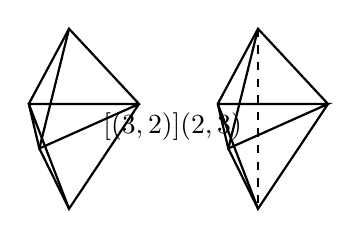
\begin{tikzpicture}[scale=1]
 \def\a{1.40}
 \def\b{0.5}
 \def\trigConst{0.816497}

 \begin{scope} [x     = {(1cm,0)},
   y     = {({0.7cm*cos(135)},{-0.7cm*sin(135)})},
   z     = {(0,1cm)}]


  \path coordinate (T1) at ({-(\b + (0.5*\a))}, {0.3333*\trigConst*\a}, {\trigConst*\a})
  coordinate (A1) at ({-\b},0,0)
  coordinate (B1) at ({-(\a + \b)},0,0)
  coordinate (C1) at ({-(\b + (0.5*\a))},{\trigConst*\a},0)
  coordinate (E1) at ({-(\b + (0.5*\a))}, {0.3333*\trigConst*\a}, {-\trigConst*\a});


  \path coordinate (T2) at ({(\b + (0.5*\a))}, {0.3333*\trigConst*\a}, {\trigConst*\a})
  coordinate (A2) at ({\b},0,0)
  coordinate (B2) at ({(\a + \b)},0,0)
  coordinate (C2) at ({(\b + (0.5*\a))},{\trigConst*\a},0)
  coordinate (D2) at ({(\b + (0.5*\a))}, {0.3333*\trigConst*\a}, {0.3333*\trigConst*\a})
  coordinate (E2) at ({(\b + (0.5*\a))}, {0.3333*\trigConst*\a}, {-\trigConst*\a});


  \draw[thick]  (A1)  -- (B1) -- (C1) -- (A1) -- (T1) -- (B1) -- (E1) -- (A1);
  \draw[thick]  (T1) -- (C1) -- (E1);

  \draw[thick]  (A2)  -- (B2) -- (C2) -- (A2) -- (T2) -- (B2) -- (E2) -- (A2);
  \draw[thick]  (T2) -- (C2) -- (E2);

  \draw[thick, dashed] (T2) -- (E2);


  \node[align=center] at ({0.15*\a},{0.5*\trigConst*\a},0) {$\xrightleftharpoons[(3,2)]{(2,3)}$};

 \end{scope}
\end{tikzpicture}

    \end{block}}
  \end{column}
 \end{columns}
 \center{\tiny{as e.g. found in INSERT SOURCE}}
 %https://arxiv.org/pdf/1412.8247.pdf
\end{frame}

\begin{frame}{Problems in four Dimensions}
 \begin{columns}[onlytextwidth,t]
  \begin{column}{0.48\textwidth}
   \begin{block}{Causal constraint (CDT)}
    \vspace{0pt}
   \end{block}
  \end{column}
  \begin{column}{0.48\textwidth}
   \begin{block}{Non trivial measure term}
    \vspace{0pt}
    Include non trivial measure term (SOURCE)
    \begin{align*}
     Z_E = \sum_T \frac{1}{C_T} \left[ \prod_{j=1}^{N_2} \mathcal{O} \left( t_j \right)^\beta \right] \mathrm{e}^{-S_E}
    \end{align*}
    with $\beta \neq 0$.
    \begin{itemize}
     \item $\mathcal{O}(t_j)$ is the \# 4-simplices the triangle $t_j$ belongs to
     \item Discrete limit of $\displaystyle \left[ \mathrm{det} (-g) \right]^{\beta/2}$
     \item Treat $\beta$ as another bare parameter
    \end{itemize}
   \end{block}
  \end{column}
 \end{columns}
\end{frame}
